\documentclass[preprint,10pt]{sigplanconf}
% \documentclass[onecolumn]{sigplanconf-onecolumn}
\usepackage[utf8]{inputenc}
\usepackage[T1]{fontenc}
\usepackage{fixltx2e}
\usepackage{graphicx}
\usepackage{longtable}
\usepackage{float}
\usepackage{wrapfig}
\usepackage{soul}
\usepackage{textcomp}
\usepackage{marvosym}
\usepackage{latexsym}
\usepackage{amssymb}
\usepackage{hyperref}
\tolerance=1000
\usepackage{amsmath}
\usepackage{amsthm}
\usepackage{stmaryrd}
\usepackage{amssymb}
\usepackage{gastex}
\usepackage{graphics}
\usepackage{listings}
\usepackage{microtype}
\usepackage{mathtools}
\usepackage{color}
\definecolor{lightgray}{rgb}{.9,.9,.9}
\definecolor{darkgray}{rgb}{.4,.4,.4}
\definecolor{purple}{rgb}{0.65, 0.12, 0.82}


% ---------------------------------------------------------------------	%
% Horizontal brackets.							%
% ---------------------------------------------------------------------	%

\newcommand{\hbra}{
\hbox to \textwidth{\vrule width0.3mm height 1.8mm depth-0.3mm
                    \leaders\hrule height1.8mm depth-1.5mm\hfill
                    \vrule width0.3mm height 1.8mm depth-0.3mm}}
\newcommand{\hket}{
\hbox to \textwidth{\vrule width0.3mm height1.5mm
                    \leaders\hrule height0.3mm\hfill
                    \vrule width0.3mm height1.5mm}}


\renewcommand{\hbra}{
\hbox to \columnwidth{\vrule width0.3mm height 1.8mm depth-0.3mm
                    \leaders\hrule height1.8mm depth-1.5mm\hfill
                    \vrule width0.3mm height 1.8mm depth-0.3mm}}
\renewcommand{\hket}{
\hbox to \columnwidth{\vrule width0.3mm height1.5mm
                    \leaders\hrule height0.3mm\hfill
                    \vrule width0.3mm height1.5mm}}


%\newcounter{figure}

% \newenvironment{proof}%
%   {%\begin{quote}
%     %\item[]
% %   \begin{quote}
%      \normalsize{\sc Proof:}\hspace*{0mm}
% }
%   {\proofcomplete
% %\end{quote}%
% \smallskip 
%    }


\newcommand{\proofcomplete}{ %\hspace*{\fill}
$\square$
}


\newenvironment{display}[1]{
  \refstepcounter{figure}
 % \begin{tabbing}
 % \hspace{1.5em} \= \hspace{.40\linewidth - 2em} \= \hspace{2em} \= \kill
%  \medskip
\noindent
  \textbf{Figure~\thefigure:  #1}\\
  \hbra\\[-.8ex]
  \nopagebreak
  %\small
 }{ 
 \\[-2ex]
 \nopagebreak
  \hket
  \nopagebreak
% \medskip
 % \end{tabbing}
 }


\newcommand{\htbra}{
\hbox to \textwidth{\vrule width0.3mm height 1.8mm depth-0.3mm
                    \leaders\hrule height1.8mm depth-1.5mm\hfill
                    \vrule width0.3mm height 1.8mm depth-0.3mm}}
\newcommand{\htket}{
\hbox to \textwidth{\vrule width0.3mm height1.5mm
                    \leaders\hrule height0.3mm\hfill
                    \vrule width0.3mm height1.5mm}}


\newenvironment{displayfigure}[1]{
  \begin{figure}[tp]
  \refstepcounter{figure}
  \medskip
  \textbf{Figure~\thefigure:  #1}\\
  \hbra\\[-.8ex]
  \nopagebreak
  %\small
 }{ 
  \\[-.8ex]
 \nopagebreak
  \hket
  \nopagebreak
 \medskip
  \end{figure}
 % \end{tabbing}
 }

\newenvironment{displayfigure*}[1]{
  \begin{figure*}[tph!]
   \refstepcounter{figure}
 \medskip
  \textbf{Figure~\thefigure:  #1}\\
  \htbra\\[-.8ex]
  \nopagebreak
%  \footnotesize
 }{ 
  \\[-.8ex]
 \nopagebreak
  \htket
  \nopagebreak
 \medskip
  \end{figure*}
 % \end{tabbing}
 }

\newenvironment{displayname}[1]{
  \refstepcounter{figure}
  \begin{tabbing}
  \hspace{1.5em} \= \hspace{.40\linewidth - 2em} \= \hspace{2em} \= \kill
  \textbf{Figure~\thefigure: #1}\\[-.8ex]
  \hbra\\[-.8ex]
  \nopagebreak
 }{
  \\[-.8ex]\hket

  \end{tabbing}
 }

%%%%%%%% typesetting type rules %%%%%%%%%%%%%
\newenvironment{trules}
{\[\begin{array}{@{}c@{}r@{}}}
{\end{array}\]}
\newcommand{\headtrule}[2]{
	\multicolumn{2}{@{}l@{}}{\mbox{#2}} \hfil \fbox{#1}\\
	\multicolumn{2}{@{}l@{}}{\hskip3.25in}\\
}
\newcommand{\trule}[3]{
\frac 
	{\strut\begin{array}{@{}c@{}} #2 \end{array}} 
	{\strut\begin{array}{@{}c@{}} #3 \end{array}}
&\rel{#1} \\~\\
}
\newcommand{\rtrule}[3]{  % restatement in proof
Suppose $#3$ via the rule:
\[
\frac 
	{\strut\begin{array}{@{}c@{}} #2 \end{array}} 
	{\strut\begin{array}{@{}c@{}} #3 \end{array}}
\qquad\rel{#1}
\]
}
\newcommand{\trulespc}[4]{
\frac 
	{\strut\begin{array}{@{}c@{}} #2 \end{array}} 
	{\strut\begin{array}{@{}c@{}} #3 \end{array}}
#4
&\rel{#1} \\~\\
}
\newcommand{\trulenoname}[2]{
\frac 
	{\strut\begin{array}{@{}c@{}} #1 \end{array}} 
	{\strut\begin{array}{@{}c@{}} #2 \end{array}}
}
\newcommand{\nrln}[3]{
\mbox{
$\begin{array}{l}
\rel{#1} \\
\quad\frac 
	{\strut\begin{array}{c} #2 \end{array}} 
	{\strut\begin{array}{c} #3 \end{array}}
\end{array}
$}}
\newcommand{\rel}[1]{\raisebox{0ex}[0ex][0ex]{\small [\textsc{#1}}]}
\newcommand{\mydefhead}[2]{\multicolumn{2}{l}{{#1}}&\mbox{\emph{#2}}\\}
\newcommand{\mydefcase}[2]{\qquad& #1 &\mbox{#2}\\}
\newcommand{\headrule}[2]{\multicolumn{3}{@{}l}{\mbox{#2}} & \fbox{#1}\\}


\newcommand{\eg}{e.g.\ }
\newcommand{\ie}{i.e.\ }

\newcommand{\num}{\textit{num}}
\newcommand{\str}{\textit{str}}

\newcommand{\Tok}{\textit{Token}}
\newcommand{\TT}{\textit{TokenTree}}

\newcommand{\tok}{\texttt{tok}}

\newcommand{\cons}[2]{#1 \cdot #2}
\newcommand{\readfn}[3]{\textrm{read}(#1,~#2,~#3)}

\newtheorem{theorem}{Theorem}
\newtheorem{lemma}{Lemma}

\newcommand{\gprod}[2]{\textit{#1}_{#2}}

\newcommand{\re}{\texttt{/} \cdot \texttt{x} \cdot \texttt{/}}
\newcommand{\rett}{\texttt{/}x\texttt{/}}
% \newcommand{\re}{\texttt{/x/}}

\newcommand{\var}{\texttt{x}}

\newcommand{\call}[2]{#1 \texttt{(}#2\texttt{)}}
\newcommand{\ifstate}[2]{\texttt{if}~\texttt{(}#1\texttt{)}#2}
\newcommand{\ifelsestate}[3]{\texttt{if}~\texttt{(}#1\texttt{)}#2~\texttt{else}#3}
\renewcommand{\div}{\texttt{/}}
\newcommand{\plus}{\texttt{+}}

\newcommand{\rcurly}{
	\underline{
		\texttt{\{}
	}
}

\newcommand{\parens}[1]{\underline{ \texttt{(} #1 \texttt{)}}}
% \newcommand{\parens}[1]{\underline{(#1)}}
\newcommand{\curlies}[1]{\underline{ \texttt{\{} #1 \texttt{\}} } }
% \newcommand{\curlies}[1]{\underline{ \{ #1 \} } }
\newcommand{\brackets}[1]{\texttt{[}#1\texttt{]}}

\newcommand{\vtok}{s}
\newcommand{\isobject}{\textrm{isExprPrefix}}
\newcommand{\reprefix}{\textit{RegexPrefix}}
\newcommand{\divprefix}{\textit{DividePrefix}}

\newcommand{\true}{\textit{true}}
\newcommand{\false}{\textit{false}}

\newcommand{\littt}[1]{\textit{<}\textit{lit}:~#1\textit{>}}
\newcommand{\addtt}[3]{\textit{<}\textit{op}:~#1,~\textit{l}:~#2,~\textit{r}:~#3\textit{>}}


\renewcommand{\verb}{\lstinline}



\authorinfo{Tim Disney}{UC Santa Cruz}{}
\authorinfo{Nathan Faubion}{Flow Corp.}{}
\authorinfo{David Herman}{Mozilla Corp.}{}
\authorinfo{Cormac Flanagan}{UC Santa Cruz}{}
\renewcommand{\author}[1]{}
\author{Tim Disney}
\date{\today}
\title{Sweeten Your JavaScript: Hygienic Macros for ES5}
\hypersetup{
  pdfkeywords={},
  pdfsubject={Sweet.js - Macros for JavaScript}}
\begin{document}


\lstdefinelanguage{JavaScript}{
  keywords={macro, typeof, new, true, false, catch, function, return, null, catch, switch, var, if, in, while, do, else, case, break},
  keywordstyle=\color{black}\textbf,
  ndkeywords={class, export, boolean, throw, implements, import, this},
  ndkeywordstyle=\color{black},
  identifierstyle=\color{black},
  sensitive=false,
  comment=[l]{//},
  morecomment=[s]{/*}{*/},
  commentstyle=\color{darkgray}\ttfamily,
  morestring=[b]',
  morestring=[b]"
}


\lstset{
   language=JavaScript,
   extendedchars=true,
   % basicstyle=\ttfamily,
   basicstyle=\footnotesize\ttfamily,
   showstringspaces=false,
   showspaces=false,
   numberstyle=\footnotesize,
   numbersep=9pt,
   tabsize=2,
   breaklines=true,
   showtabs=false,
   captionpos=b
}


\maketitle

\abstract{ Lisp and Scheme have demonstrated the power of macros to
  enable programmers to evolve and craft languages. In languages with
  more complex syntax, macros have had less success. In part, this has
  been due to the difficulty in building expressive hygienic macro
  systems for such languages. JavaScript in particular presents unique
  challenges for macro systems due to ambiguities in the lexing stage
  that force the JavaScript lexer and parser to be intertwined.

  In this paper we present a novel solution to the lexing ambiguity of
  JavaScript that enables us to cleanly separate the JavaScript lexer
  and parser by recording enough history during lexing to resolve
  ambiguities. We give an algorithm for this solution along with a
  proof that it does in fact correctly resolve ambiguities in the
  language. Though the algorithm and proof we present is specific to
  JavaScript, the general technique can be applied to other languages
  with ambiguous grammars.
  With lexer and parser separated, we then implement
  an expressive hygienic macro system for JavaScript called sweet.js.
}

\section{Introduction}
\label{sec-1}

\begin{displayfigure*}{\label{fig:editor}The sweet.js editor}

\centering
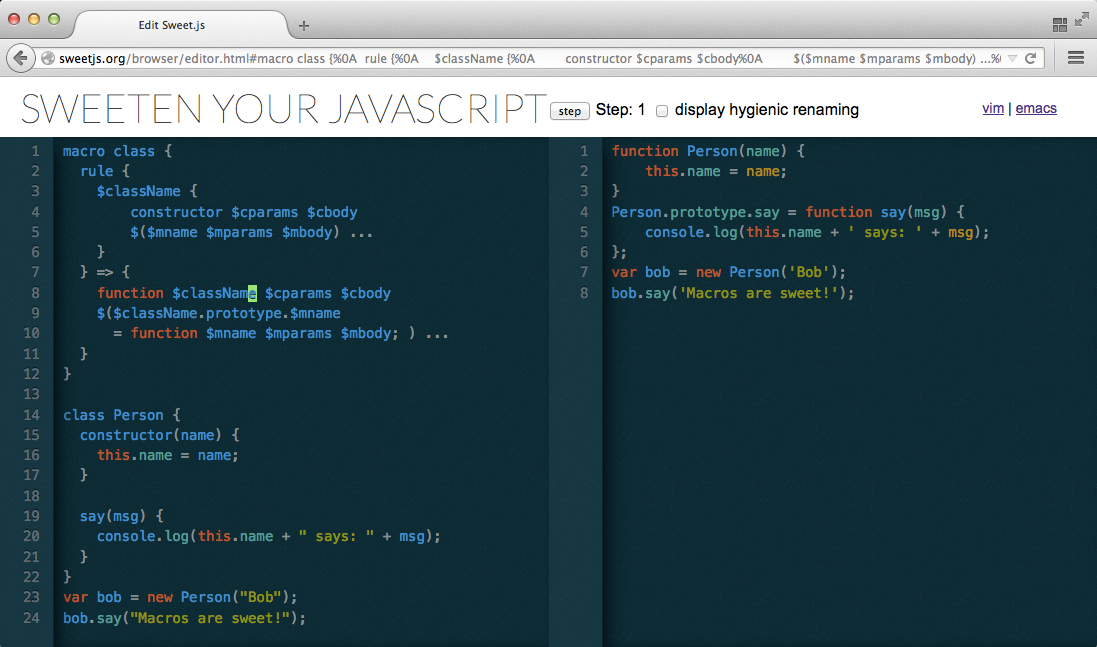
\includegraphics[scale=0.44]{sweetjs_browser.png}
\end{displayfigure*}

Expressive macro systems have a long history in the design of
extensible programming languages going back to Lisp and Scheme
\cite{Kohlbecker1987,Foderaro1983} as a powerful tool that enables
programmers to craft their own languages.

While macro systems have found success in many Lisp-derived languages,
they have not been widely adopted in languages such as JavaScript. In
part, this failure is due to the difficulty of implementing macro
systems for languages without fully delimited s-expressions. A key
feature of a sufficiently expressive macro system is the ability for
macros to manipulate unparsed and unexpanded subexpressions. In a
language with parentheses like Scheme, manipulating unparsed
subexpressions is simple:
\begin{lstlisting}
(if (> denom 0)
    (/ x denom)
    (error "divide by zero"))
\end{lstlisting}
The Scheme \emph{reader} converts the source string into nested
s-expressions, which macros can easily manipulate. Since each
subexpression of the \verb!if! form is a fully delimited
s-expression, it is easy to implement \verb!if! as a
macro.

% A language with richer syntax like JavaScript complicates this
% process:
% \begin{lstlisting}
% if (denom > 0)
%   x / denom;
% else
%   throw "divide by zero";
% \end{lstlisting}
% Without fully parsing, it is difficult to know where 

Conceptually, the Scheme compiler lexes a source string into
a stream of tokens which are then read into s-expressions
before being macro expanded and parsed into an abstract syntax tree.
\[
\textit{lexer} \xrightarrow{\textit{Token}^{*}}
\textit{reader} \xrightarrow{\textit{Sexpr}}
\textit{expander/parser} \xrightarrow{\textit{AST}}
\]

As a first step to designing a Scheme-like macro system for
JavaScript, it is necessary to introduce a read step into the compiler
pipeline. However, the design of a correct reader for full JavaScript
turns out to be surprisingly subtle, due to ambiguities in how regular
expression literals (such as \verb!/[0-9]*/!) and the divide
operator (\verb!/!) should be lexed. In traditional JavaScript
compilers, the parser and lexer are intertwined. Rather than run the
entire program through the lexer once to get a sequence of tokens, the
parser calls out to the lexer from a given grammatical context with a
flag to indicate if the lexer should accept a regular expression or
a divide operator, and the input character stream is tokenized accordingly.
So if the parser is in a context that accepts a regular expression, the characters ``\verb!/x/!'' will be lexed into the single token \underline{\verb!/x/!} otherwise it will lex into the individual tokens \underline{\verb!/!}, \underline{\verb!x!}, and \underline{\verb!/!}.
\[
\textit{lexer} \xleftrightharpoons[\textit{Token}^{*}]{\textit{feedback}}
\textit{parser} \xrightarrow{\textit{AST}}
\]
It is necessary to separate the parser and lexer in order to implement
a macro system for JavaScript. Our JavaScript macro system,
sweet.js, includes a separate
reader that converts a sequence of tokens into a sequence of token
trees (a little analogous to s-expressions) without feedback from the
parser.
\[
\textit{lexer} \xrightarrow{\textit{Token}^{*}}
\textit{reader} \xrightarrow{\textit{TokenTree}^{*}}
\textit{expander/parser} \xrightarrow{\textit{AST}}
\]
This enables us to finally separate the JavaScript lexer and parser
and build a fully hygienic macro system for JavaScript. The reader
records sufficient history information in the form of token trees in
order to correctly decide whether to parse a sequence of tokens
\verb!/x/g! as a regular expression or as division operators (as in
\verb!4.0/x/g!). Surprisingly, this history information needs to be
remembered from arbitrarily far back in the token stream.

While the algorithm for resolving ambiguities we present in this paper
is specific to JavaScript, the technique of recording history in the
reader with token trees can be applied to other languages with
ambiguous grammars.
% We expand on this point in
% Section~\ref{sec:discussion}.

Once JavaScript source has been correctly read, there are still a
number of challenges to building an expressive macro system. The lack
of parentheses in particular make writing declarative macro
definitions difficult. For example, the \verb!if! statement in
JavaScript allows undelimited then and else branches:
\begin{lstlisting}
if (denom > 0)
  x / denom;
else
  throw "divide by zero";
\end{lstlisting}
It is necessary to know where the then and else branches end to
correctly implement an \verb!if! macro but this is complicated by
the lack of delimiters. 

The solution to this problem that we take is by progressively building
a partial AST during macro expansion. Macros can then match against
and manipulate this partial AST. For example, an \verb!if! macro
could indicate that the then and else branches must be single
statements and then manipulate them appropriately.


This approach, called \emph{enforestation}, was pioneered by Honu
\cite{Rafkind2012,Rafkind2013}, which we adapt here for
JavaScript\footnote{The syntax of Honu is similar to JavaScript but does
  not support regular expression literals, which simplifies their
  reader. }. In addition, we make two extensions to the Honu technique
that enable more expressive macros to be built. First, as described in
Section \ref{sec:infix} we add support for infix macros, which allow
macros to match syntax both before and after the macro identifier.
Secondly, we implement the \verb!invoke! pattern class, described in
Section \ref{sec:invoke}, which allows macro authors to extend the
patterns used to match syntax.

Sweet.js is implemented in JavaScript and takes source code written with sweet.js macros and produces the expanded source that can be run in any JavaScript environment. 
The project web page\footnote{\url{http://sweetjs.org}} includes an interactive browser-based editor that makes it simple to try out writing macros without requiring any installation.
Figure \ref{fig:editor} shows the editor in action; a macro implementing classes is being edited in the left pane and the right pane continually shows the expanded output.
There is already an active community using sweet.js to, for example, implement
significant features from the upcoming ES6 version of JavaScript \cite{Long} or implement pattern matching in JavaScript \cite{Faubion}.

% This paper we present a reader implementation that addresses the complexities of JavaScript (Section \ref{sec:read}), including regular expression literals, together with a correctness proof (Section \ref{sec:provingread}) for this reader.
% We also describe our implementation of a hygienic macro system for JavaScript (Sections \ref{sec:writingMacros} and \ref{sec:enforest}) which includes
% the ability to define infix macros (Section \ref{sec:infix}) that match on arbitrary surrounding syntax and
%  the \texttt{invoke} primitive (Section \ref{sec:invoke}) to allow custom parser classes and more powerful matching.



\section{Reading JavaScript}
\label{sec:read}


\begin{displayfigure}{\label{fig:ast}AST for Simplified JavaScript}
\[
\begin{array}{rrl}
  e \in \textit{AST} &::=& x ~|~ \rett ~|~ 
  \texttt{\{} 
  \var
  \texttt{:}
  ~e
  \texttt{\}}
  ~|~ \texttt{(} e \texttt{)}
  ~|~ e\texttt{.}\var ~|~ e \texttt{(} e \texttt{)}
  \\
  &|& e~\div~e ~|~ e ~\texttt{+}~ e ~|~ e ~\texttt{=}~ e
  ~|~ \texttt{\{} e \texttt{\}} ~|~ \var \texttt{:} e ~|~ \texttt{if}~
  \texttt{(} e \texttt{)}~e
  \\ 
  &|& \texttt{return} ~|~ \texttt{return}~e
  \\
  &|& \texttt{function}~x~
  \texttt{(}x \texttt{)}~
  \texttt{\{} e \texttt{\}} ~|~ e~e
\end{array}
\]
\end{displayfigure}


\begin{displayfigure*}{\label{fig:simpleread}Simplified Read Algorithm}
\begin{minipage}[t]{0.5\linewidth}
\[
\begin{array}{lrl}
  \textit{Punctuator} &::=& \div ~|~ \texttt{+} ~|~ \texttt{:} ~|~
  \texttt{;} ~|~ \texttt{=} ~|~ \texttt{.}
  \\
  \textit{Keyword} &::=& \texttt{return} ~|~ \texttt{function}~|~
  \texttt{if}
  \\


   \Tok &::=& x ~|~ \textit{Punctuator} ~|~ \textit{Keyword}
  \\
  &|& 
  \texttt{\{} ~|~ 
  \texttt {\}} ~|~  
  \texttt{(} ~|~ 
  \texttt{)}
  \\
  k \in \TT &::=& x ~|~ \textit{Punctuator} ~|~ \textit{Keyword}
  \\
  &|& \rett ~|~ \parens{t} ~|~ \curlies{t}
  \\
  r \in \textit{RegexPat} &::=& x ~|~ \texttt{\{} ~|~ \texttt{\}}
  ~|~ \texttt{(} ~|~ \texttt{)}
  \\
  x &\in& \textit{Variable}
  \\
  s &\in& \Tok^{*}
  \\
  t,p &\in& \TT^{*}
\end{array}
\]
\end{minipage}
\begin{minipage}[t]{0.5\linewidth}
\[
  \begin{array}{lcll}
    \multicolumn{3}{l}{\textrm{isExprPrefix} : \TT^{*} \rightarrow
      \textit{Bool} \rightarrow \textit{Int} \rightarrow \textit{Bool}}
    \\
    \isobject(\epsilon,~\textit{true},~l) &=& \textit{true}
    \\
    \isobject(p \cdot \div,~b,~l) &=& \textit{true}
    \\
    \isobject(p \cdot \texttt{+},~b,~l) &=& \textit{true}
    \\
    \isobject(p \cdot \texttt{=},~b,~l) &=& \textit{true}
    \\
    \isobject(p \cdot \texttt{:},~b,~l) &=& b
    \\
    \isobject(p \cdot \texttt{return}^{l},~b,~l') &=& \textit{false} 
    & \textit{if}~l \not = l'
    \\
    \isobject(p \cdot \texttt{return}^{l},~b,~l') &=& \textit{true} 
    & \textit{if}~l = l'
    \\
    \isobject(p ,~b,~l) &=& \textit{false}
    \\
  \end{array}
\]
\end{minipage}
\[
  \begin{array}{lcll}
    \multicolumn{3}{l}{\textrm{read} : \Tok^{*} \rightarrow \TT^{*}
      \rightarrow \textit{Bool} \rightarrow \TT^{*}}
    \\
    % regex
    \readfn{/\cdot r \cdot /\cdot \vtok}{\epsilon}{b}
    &=&
    \cons{/r/}{
      \readfn{\vtok}{/r/}{b}
    }
    \\
    \readfn{/\cdot r \cdot /\cdot \vtok}{p \cdot k}{b}
    &=&
    \cons{/r/}{
      \readfn{\vtok}{
        p \cdot k \cdot /r/
      }{b}
    }
    \\
    \quad\textit{if}~k \in \textit{Punctuator} \cup \textit{Keyword}
    \\
    \readfn{/\cdot r \cdot /\cdot \vtok}{
      p \cdot \texttt{if} \cdot \parens{t}
    }{b}
    &=&
    \cons{/r/}{
      \readfn{\vtok}{p \cdot \texttt{if} \cdot \parens{t} \cdot /r/}{b}
    }
    \\
    \readfn{/\cdot r \cdot /\cdot \vtok}{
      p \cdot \texttt{function}^{l} \cdot x
      \cdot \parens{t} \cdot \curlies{t'}
    }{b}
    &=&
    \cons{/r/}{
      \readfn{\vtok}{
      p 
      \cdot \texttt{function}^{l} \cdot x \cdot 
      \parens{t} \cdot \curlies{t'}\cdot /r/
      }{b}
    } \\
    \quad \textit{if}~\isobject(p,~b,~l) = \false
    \\
    \readfn{/\cdot r \cdot / \cdot \vtok}{
      p \cdot \curlies{t}^{l}
    }{b}
    &=&
    \cons{/r/}{
      \readfn{\vtok}{
        p \cdot \curlies{t}^{l}\cdot /r/
      }{b}
    }
    \\
    \quad \textit{if}~ \isobject(p,~b,~l) = \false

    \\ \\

    % divide
    \readfn{/\cdot \vtok}{p\cdot x}{b}
    &=&
    \cons{/}{
      \readfn{\vtok}{
        p\cdot x\cdot /
      }{b}
    }
    \\
    \readfn{/\cdot \vtok}{p \cdot /x/}{b}
    &=&
    \cons{/}{
      \readfn{\vtok}{
        p \cdot /x/ \cdot /
      }{b}
    }
    \\
    \readfn{/\cdot \vtok}{p \cdot \parens{t}}{b}
    &=&
    \cons{/}{
      \readfn{\vtok}{
        p \cdot \parens{t} \cdot /
      }{b}
    }
    \\
    \readfn{/\cdot \vtok}{
      p  \cdot \texttt{function}^l \cdot x
      \cdot \parens{t} \cdot \curlies{t'}
    }{b}
    &=&
    \cons{/}{
      \readfn{\vtok}{
        p  \cdot \texttt{function}^l \cdot x \cdot \parens{t}
        \cdot \curlies{t'} \cdot /
      }{b}
    }
    \\
    \quad \textit{if}~\isobject(p,~b,~l)= \true
    \\
    \readfn{/\cdot \vtok}{
      p \cdot \curlies{t}^{l}
    }{b}
    &=&
    \cons{/}{
      \readfn{\vtok}{
        p \cdot \curlies{t}^{l} \cdot /
      }{b}
    }
    \\
    \quad \textit{if}~\isobject(p,~b,~l)= \true

    \\ \\
    

    % other
    \readfn{\texttt{(} \cdot \vtok \cdot \texttt{)} \cdot \vtok'}{p}{b}
    &=&
    \cons{\parens{t}}{
      \readfn{\vtok'}{p \cdot \parens{t}}{b}
    } 
    \\
    \quad \textit{where}~s~\textit{contains no unmatched}~\texttt{)} 
    &&\quad \textit{where}~t = \readfn{s}{\epsilon}{\textit{false}} 
    \\
    \readfn{
      \texttt{\{}^l \cdot \vtok \cdot \texttt{\}} \cdot \vtok'
    }{p}{b}
    &=&
    \cons{\curlies{t}^l}{
      \readfn{\vtok'}{
        p \cdot \curlies{t}^l
      }{b}
    } 
    \\
    \quad \textit{where}~s~\textit{contains no unmatched}~\texttt{\}} 
    && \textit{where}~t = \readfn{s}{\epsilon}{\isobject(p,~b,~l)}
    \\
    \readfn{x \cdot \vtok}{p}{b}
    &=&
    \cons{x}{
      \readfn{\vtok}{p \cdot x}{b}
    }
    \\
    \readfn{\epsilon}{p}{b}
    &=&
    \epsilon \\
  \end{array}
\]
\end{displayfigure*}

\begin{displayfigure*}{\label{fig:grammar}Simplified ES5 Grammar}
\[
\begin{array}{lcl}
  \gprod{PrimaryExpr}{x} &::=& x
  \\
  \gprod{PrimaryExpr}{\rett} &::=& \texttt{/} \cdot x \cdot \texttt{/}
  \\
  \gprod{PrimaryExpr}{
    \texttt{\{} \var \texttt{:} e \texttt{\}}
  } 
  &::=& 
  \texttt{\{} \cdot \var \cdot \texttt{:} \cdot  \gprod{AssignExpr}{e}
    \cdot \texttt{\}}
  \\
  \gprod{PrimaryExpr}{\texttt{(} e \texttt{)}} &::=& 
  \texttt{(} \cdot \gprod{AssignExpr}{e} \cdot \texttt{)}
  \\ \\
  \gprod{MemberExpr}{e} &::=&
  \gprod{PrimaryExpr}{e}
  \\
  \gprod{MemberExpr}{e} &::=&
  \gprod{Function}{e}
  \\
  \gprod{MemberExpr}{e\texttt{.\var}} &::=&
  \gprod{MemberExpr}{e} \cdot \texttt{.} \cdot \var
  \\ \\
  \gprod{CallExpr}{e~ \texttt{(}e' \texttt{)}} &::=& 
  \gprod{MemberExpr}{e} \cdot
  \texttt{(}\cdot \gprod{AssignExpr}{e'} \cdot \texttt{)}
  \\
  \gprod{CallExpr}{e~ \texttt{(}e' \texttt{)}} &::=& 
  \gprod{CallExpr}{e} \cdot
  \texttt{(}\cdot \gprod{AssignExpr}{e'} \cdot \texttt{)}
  \\
  \gprod{CallExpr}{e\texttt{.\var}} &::=& 
  \gprod{CallExpr}{e}~\texttt{.}~
  \var
  \\ \\
  \gprod{BinaryExpr}{e} &::=& \gprod{CallExpr}{e} \\
  \gprod{BinaryExpr}{e ~\div~ e'}
  &::=&
  \gprod{BinaryExpr}{e} \cdot \div \cdot  \gprod{BinaryExpr}{e'} \\
  \gprod{BinaryExpr}{e ~\plus~ e'}
  &::=&
  \gprod{BinaryExpr}{e} \cdot \plus \cdot \gprod{BinaryExpr}{e'}
  \\ \\
  \gprod{AssignExpr}{e} &::=&
  \gprod{BinaryExpr}{e}
  \\
  \gprod{AssignExpr}{e~\texttt{=}~e'} &::=&
  \gprod{CallExpr}{e} \cdot \texttt{=} \cdot
  \gprod{AssignExpr}{e'}
  \\ \\
  \gprod{StmtList}{e} &::=&
  \gprod{Stmt}{e}
  \\
  \gprod{StmtList}{e~e'} &::=&
  \gprod{StmtList}{e} \cdot
  \gprod{Stmt}{e'}
  \\ \\
  \gprod{Stmt}{\texttt{\{} e \texttt{\}}} &::=& 
  \texttt{\{} \cdot \gprod{StmtList}{e}\cdot \texttt{\}}
  \\
  \gprod{Stmt}{\var\texttt{:}~e} &::=&
  \var\cdot \texttt{:}\cdot\gprod{Stmt}{e}
  \\
  \gprod{Stmt}{e} &::=& 
  \gprod{AssignExpr}{e} \cdot \texttt{;}
  \qquad \textit{where lookahead}~\not = 
    \texttt{\{}~\textit{or}~\texttt{function}
  \\
  \gprod{Stmt}{\texttt{if}~\texttt{(}e \texttt{)}~e'} &::=& 
  \texttt{if}\cdot 
  \texttt{(}\cdot \gprod{AssignExpr}{e} \cdot \texttt{)}\cdot \gprod{Stmt}{e'}
  \\
  \gprod{Stmt}{\texttt{return}} &::=& 
  \texttt{return}
  \\
  \gprod{Stmt}{\texttt{return}~e} &::=& 
  \texttt{return}\cdot \textrm{[no line terminator
    here]}~\gprod{AssignExpr}{e}\cdot \texttt{;}
  \\ \\
  \gprod{Function}{\texttt{function}~x~ \texttt{(}x' \texttt{)}~\texttt{\{}e \texttt{\}}} 
  &::=&
  \texttt{function} \cdot x \cdot 
  \texttt{(} \cdot x' \cdot \texttt{)}\cdot
  \texttt{\{}\cdot \gprod{SourceElements}{e} \cdot \texttt{\}}
  \\ \\
  \gprod{SourceElement}{e} &::=& \gprod{Stmt}{e} 
  \\
  \gprod{SourceElement}{e} &::=& \gprod{Function}{e}
  \\ \\

  \gprod{SourceElements}{e} &::=& \gprod{SourceElement}{e}
  \\
  \gprod{SourceElements}{e~e'} &::=&
  \gprod{SourceElements}{e}\cdot \gprod{SourceElement}{e'}
  \\ \\
  \gprod{Program}{e} &::=& \gprod{SourceElements}{e}
  \\
  \gprod{Program}{} &::=& \epsilon
\end{array}
\]  
\end{displayfigure*}

Parsers give structure to unstructured source code. In parsers without
macro systems this is usually accomplished by a lexer (which converts
a character stream to a token stream) and a parser (which converts the
token stream into an AST according to a context-free grammar). A
system with macros must implement a macro \emph{expander} that sits
between the lexer and parser. Some macros systems, such as the C
preprocessor \cite{Harbison1984}, work over just the token stream.
However, to implement truly
expressive Scheme-like macros that can manipulate groups of unparsed
tokens, it is necessary to structure the token stream via a
\emph{reader}, which performs delimiter matching and enables macros to manipulate delimiter-grouped tokens.

As mentioned in the introduction, the design of a correct reader for JavaScript is surprisingly subtle due to ambiguities between lexing regular expression literals and the divide operator. This disambiguation is critical to the correct implementation of read because delimiters can appear inside of a regular expression literal. If the reader failed to distinguish between a regular expression/divide operator, it could result in incorrectly matched delimiters. 
\begin{lstlisting}
function makeRegex() {
  // results in a parse error if the
  // first / is incorrectly read as divide
  return /}/;
}
\end{lstlisting}

A key novelty in sweet.js is the design and implementation of a reader
that correctly distinguishes between regular expression literals and
the divide operator for full ES5 JavaScript\footnote{Our
  implementation also has initial support for code written in the
  upcoming ES6 version of JavaScript.}. For clarity of presentation,
this paper describes the implementation of read for the subset of
JavaScript shown in Figure \ref{fig:grammar}, which retains the
essential complications of the full version of read.

\subsection{Formalism}

In our formalism in Figure \ref{fig:simpleread}, read takes a \textit{Token} sequence. Tokens are the output of a very simple lexer, which we do not define here. This lexer does not receive feedback from the parser like the ES5 lexer does, and so does not distinguish between regular expressions and the divide operator. Rather it simply lexes slashes into the ambiguous \texttt{/} token. Tokens also include keywords, puncutators, the (unmatched) delimiters, and variable identifiers.
\[
\begin{array}{lrl}
  \textit{Punctuator} &::=& \div ~|~ \texttt{+} ~|~ \texttt{:} ~|~
  \texttt{;} ~|~ \texttt{=} ~|~ \texttt{.}
  \\
  \textit{Keyword} &::=& \texttt{return} ~|~ \texttt{function}~|~ \texttt{if}
  \\
  \Tok &::=& x ~|~ \textit{Punctuator} ~|~ \textit{Keyword}
  \\
  &|& 
  \texttt{\{} ~|~ 
  \texttt {\}} ~|~  
  \texttt{(} ~|~ 
  \texttt{)}
  \\
  x, y &\in& \textit{Variable}
  \\
  s &\in& \Tok^{*}
 \end{array}
\]

The job of read is then to produce a correct \textit{TokenTree} sequence. Token trees include regular expression literals $\rett$, where $r$ is the regular expression body. We simplify regular expression bodies to just a variable and the individual delimiters, which captures the essential problems of parsing regular expressions.
Token trees also include fully matched delimiters with nested token tree sequences $\parens{t}$ and $\curlies{t}$ rather than individual delimiters (we write token tree delimiters with an \underline{underline} to distinguish them from token delimiters).
\[
\begin{array}{lrl}
  k \in \TT &::=& x ~|~ \textit{Punctuator} ~|~ \textit{Keyword}
  \\
  &|& \rett ~|~ \parens{t} ~|~ \curlies{t}
  \\
  r \in \textit{RegexPat} &::=& x ~|~ \texttt{\{} ~|~ \texttt{\}}
  ~|~ \texttt{(} ~|~ \texttt{)}
  \\
  t,p &\in& \TT^{*}
\end{array}
\]

Each token and token tree also carries their line number from the original source string. Line numbers are needed because there are edge cases in the JavaScript grammar 
where newlines influence parsing.
For example,
the following function returns the object literal \verb!{x: y}! as expected. 
\begin{lstlisting}
function f(y) {
  return { x: y }
}
\end{lstlisting}
However, adding a newline causes this function to 
return \verb!undefined!, because the grammar calls for an implicit semicolon to be inserted after the \verb!return! keyword.
\begin{lstlisting}
function g(y) {
  return 
  { x: y }
}
\end{lstlisting}
For clarity of presentation, we leave token line numbers implicit unless we require them, in which case we use the notation $\texttt{\{}^l$ where $l$ is a line number.

We write a token sequence by separating elements with a dot so
the source string ``\texttt{foo(/)/)}'' 
is lexed into a sequence
of six tokens \( \texttt{foo}\cdot \texttt{(} \cdot \div \cdot \texttt{)}
\cdot \div \cdot \texttt{)} \). The equivalent token tree sequence is
\(
\texttt{foo} \cdot \parens{\cdot \texttt{/} \texttt{)} \texttt{/} \cdot }
\).

\subsection{Read Algorithm}

The key idea of read is to maintain a prefix of already read token
trees. When the reader comes to a slash and needs to decide if it
should read the slash as a divide token or the start of a regular
expression literal, it consults the prefix. Looking back at most five
tokens trees in the prefix is sufficient to disambiguate the slash
token. Note that this may correspond to looking back an unbounded
distance in the original token stream.

Some of the cases of read are relatively obvious. For example, if the
token just read was one of the binary operators (\eg the \texttt{+} in
\(\texttt{f} \cdot \texttt{+} \cdot \texttt{/} 
\cdot \texttt{\}} \cdot \texttt{/}
\)) the slash will always be the start of a regular expression
literal. 

Other cases require additional context to disambiguate. For example,
if the previous token tree was a parentheses (\eg 
\(
\texttt{foo} \cdot \texttt{(} \cdot \texttt{x} \cdot \texttt{)} \cdot \texttt{/} \cdot \texttt{y}
\)
) then slash will be the divide
operator, \emph{unless} the token tree before the parentheses was the
keyword \texttt{if}, in which case it is actually the start of a
regular expression (since single statement \texttt{if} bodies do not require
braces).

\begin{lstlisting}
if (x) /}/   // regex
\end{lstlisting}

One of the most complicated cases is a slash after curly braces. Part
of the complication here is that curly braces can either indicate an
object literal (in which case the slash should be a divide) or a block
(in which case the slash should be a regular expression), but even
more problematic is that both object literals and blocks with labeled
statements can nest. For example, in the following code snippet the
outer curly brace is a block with a labeled statement \verb!x!, which
is another block with a labeled statement \verb!y! followed by a
regular expression literal.
\begin{lstlisting}
{
  x:{y: z} /}/  // regex
}
\end{lstlisting}

But if we change the code slightly, the outer curly braces become an
object literal and \verb!x! is a property so the inner curly
braces are also an object literal and thus the slash is a divide operator.

\begin{lstlisting}
o = {
  x:{y: z} /x/g  // divide
}
\end{lstlisting}

While it is unlikely that a programmer would attempt to intentionally
perform division on an object literal, it is not a parse error. In
fact, this is not even a runtime error since JavaScript will
implicitly convert the object to a number (technically
\verb!NaN!) and then perform the division (yielding
\verb!NaN!).

The reader handles these cases by checking if the prefix of a curly
brace forces the curly to be an object literal or a statement
block and then setting a boolean flag to be used while reading the
tokens inside of the braces.

Based on this discussion, our reader is implemented as
a function that takes a sequence of tokens, a prefix of previously read token trees, a boolean indicating if the token stream currently being read is inside an object literal, and returns a sequence of token trees.
\[
\textrm{read} : \Tok^{*} \rightarrow \TT^{*} 
\rightarrow \textit{Bool} \rightarrow \TT^{*}
\]

The implementation of read shown in Figure \ref{fig:simpleread} includes an auxiliary function isExprPrefix used to determine if the prefix for a curly brace indicates that the braces should be part of an expression (\ie the braces are an object literal) or if they should be a block statement.

Interestingly, the isExprPrefix function must also be used when the prefix before a slash contains a function definition. This is because there are two kinds of function definitions in JavaScript, function expressions and function declarations, and these also affect how slash is read. For example, a slash following a function declaration is always the start of a regular expression:
\begin{lstlisting}
function f() {}
/}/   // regex
\end{lstlisting}
However, a slash following a function expression is a divide operator:
\begin{lstlisting}
x = function f() { } 
/y/g   // divide
\end{lstlisting}
As in the object literal case, it is unlikely that a programmer would attempt to intentionally divide a function expression but it is not an error to do so.



\subsection{Proving Read}
\label{sec:provingread}

To show that our read algorithm correctly distinguishes 
divide operations from regular expression literals, we show that
a parser defined over normal tokens produces the same AST as a parser
defined over the token trees produced from read.

The parser for normal tokens is defined in Figure \ref{fig:grammar},
and generates ASTs in the abstract syntax shown in Figure \ref{fig:ast}. A
parser for the nonterminal \( \gprod{Program}{} \) is a function from a
sequence of tokens to an AST.
\[
\gprod{Program}{} :: \Tok^* \rightarrow \textit{AST}
\]
We use notation whereby the grammar production $\gprod{Program}{e} ::= \gprod{SourceElements}{e}$
means to match the input sequence with $\gprod{SourceElements}{e}$ and
produce the resulting AST $e$.

Note that the grammar we present here is a simplified version of the
grammar specified in the ECMAScript 5.1 standard \cite{International2011}
and many nonterminal names are shortened
versions of nonterminals in the standard.
It is mostly straightforward to extend the algorithm
presented here 
to 
the full sweet.js implementation for ES5 JavaScript.

In addition to the \( \gprod{Program}{} \) parser just described, we
also define a parser \( \gprod{Program'}{} \) that works over token
trees. The rules of the two parsers are identical, except that
all rules with delimiters and regular expression literals change as follows:
\[
\begin{array}{lcl}
  \gprod{PrimaryExpr}{\rett} &::=& \texttt{/}\cdot r \cdot \texttt{/}
  \\
  \gprod{PrimaryExpr'}{\rett} &::=& \rett
  \\
  \gprod{PrimaryExpr}{\texttt{(} e \texttt{)}} &::=& 
  \texttt{(} \cdot \gprod{AssignExpr}{e} \cdot \texttt{)}
  \\
  \gprod{PrimaryExpr'}{\texttt{(} e \texttt{)}} &::=& 
  \parens{\gprod{AssignExpr'}{e}}
  \\
\end{array}
\]

To prove that read is correct, we show that the following two parsing
strategies give identical behavior:
\begin{itemize}
\item The traditional parsing strategy takes a token sequence \( s
  \) and parses \( s \) into an AST \( e \) using the traditional parser
  \( \gprod{Program}{e} \).

\item The second parsing strategy first reads \( s \) into a token
  tree sequence \( \readfn{s}{\epsilon}{\false} \), and then parses
  this token tree sequence into an AST \( e \) via \( \gprod{Program'}{e} \).
\end{itemize}

\begin{theorem}[\label{thrm:readProgram}Parse Equivalence]\mbox{}

  \( \forall s \in \Tok^*. \)

  \( s \in \gprod{Program}{e} \Leftrightarrow 
  \readfn{s}{\epsilon}{\textit{false}} \in \gprod{Program'}{e} \)

\end{theorem}
\begin{proof}\mbox{}
  The proof proceeds by induction on ASTs to show that parse
  equivalence holds between all corresponding nonterminals in the two
  grammars. We present the details of this proof in an
  appendix available online~\cite{sweetjsappendix}.
  % Appendix \ref{sec:readproof}.
\end{proof}




\section{Writing Macros}
\label{sec:writingMacros}

The sweet.js system provides two kinds of macros: \emph{rule} macros
(analogous to \verb!syntax-rules! in Scheme \cite{Clinger1991})
and \emph{case} macros (analogous to \verb!syntax-case! in
Scheme \cite{Hieb1992}). Rule macros are the simpler of the two and work by matching
on a pattern and generating a template:

\begin{lstlisting}
macro <name> {
  rule { <pattern> } => { <template> }
}
\end{lstlisting}

For example, the following macro introduces a new function definition
form:

\begin{lstlisting}
macro def {
  rule { 
    $name ($params (,) ...) { $body ... } 
  } => {
    function $name ($params ...) {
      $body ...
    }
  }
}
def id (x) { return x; }
// expands to:
// function id (x) { return x; }
\end{lstlisting}

The pattern is matched against the syntax following the macro name.
Identifiers in a pattern that begin with \verb!$! are
\emph{pattern variables} and bind the syntax they match in the
template (identifiers that do not begin with \verb!$! are matched
literally). The ellipses (\verb!$params (,) ...!) mean match zero or more
tokens separated by commas.

The above example shows the power of matching delimited groups of
syntax (\ie matching all the tokens inside the function body). In
order for macros to be convenient in a language like JavaScript, it is
necessary to have the ability to match logical groupings of syntax
that are not fully delimited. For example, consider the
\verb!let! macro:

\begin{lstlisting}
macro let {
  rule { $id = $init:expr } => {
    var $id = $init
  }
}
let x = 40 + 2;
// expands to:
// var x = 40 + 2;
\end{lstlisting}

The initialization of a \verb!let! can be an arbitrary expression so
we use the \emph{pattern class} \verb!:expr! to greedily match the
largest possible expression, so in this example the entire expression
\verb!40 + 2! is bound to \verb!$init!.

Note that sweet.js does not provide a non-greedy form of \verb!:expr!
so there is no way, for example, to match the pattern
\verb!$x:expr + 10!. In our experience to date it appears rare to need
to match on syntax that extends an expression and so have avoided
increasing the complexity of the implementation and pattern matching
language by adding a non-greedy form.

Along with the template-based rule macros, sweet.js also provides the
more powerful procedural \emph{case} macros. 
While rule macros just provide term rewriting, case macros allow macro authors to use JavaScript code to procedurally create and manipulate syntax. 
For example, the following macro creates a string from the contents of a file.
\begin{lstlisting}
macro fromFile {
  case {_ ($path) } => {
    var fname = unwrapSyntax(#{$path});
    var f = readFile(fname);
    letstx $content = [makeValue(f, #{here})];
    return #{$content}
  }
}
var s = fromFile ("./file.txt")
// expands to:
// s = "contents of file";
\end{lstlisting}
Syntax bound in the macro pattern can be referenced inside of
JavaScript code using the notation \verb!#{ ... }!. Here we take the
file name token matched by the macro (\verb!#{$path}!), unwrap it
(like in Scheme, tokens that can be manipulated by a case macro are
represented as a \emph{syntax object} which wraps a token with its
lexical context used to maintain hygiene so unwrapping extracts just
the token), and read\footnote{Note that \verb!readFile! will depend on
  the particular JavaScript environment in which sweet.js is being run
  (\eg in node.js it might be \verb!fs.readFile! and in the browser it
  might be an \verb!XMLHttpRequest!).} the file into a variable. The
\verb!makeValue! function is used to create a string syntax object
(\verb!#{here}! is just a placeholder for the lexical context used for
hygiene) from the context of the file and \verb!letstx! (analogous to
\verb!with-syntax! in Scheme) binds that new syntax object to a
pattern variable \verb!$content! that can be used inside of a
template.

\section{Enforestation}
\label{sec:enforest}

The token tree structure produced by the reader is sufficient to
implement an expressive macro system for a fully delimited language
like Scheme. However since most of the syntax forms in a language like
JavaScript are only partially delimited, it is necessary to provide
additional structure during expansion that allows macros to manipulate
undelimited or partially delimited groups of tokens. As an example,
consider the \verb!let! macro described earlier:

\begin{lstlisting}
macro let {
  rule { $id = $init:expr } => {
    var $id = $init
  }
}
let x = 40 + 2;
// expands to:
// var x = 40 + 2;
\end{lstlisting}

Like many syntactic forms in JavaScript, the variable initialization
expression is an undelimited group of tokens. Building an expressive
macro system requires that the macro can match and manipulate patterns
such as an expression.

Sweet.js groups tokens by transforming a token tree into a \emph{term
  tree} through a technique pioneered by the Honu language called
\emph{enforestation} \cite{Rafkind2013}. Enforestation works by
progressively recognizing and grouping (potentially undelimited)
syntax forms (\eg literals, identifiers, expressions, and statements)
during expansion. Essentially, enforestation delimits undelimited
syntax.

A term tree is a kind of proto-AST that represents a partial parse of
the program. As the expander passes through the token trees, it
creates term trees that contain unexpanded sub trees that will be
expanded once all macro definitions have been discovered in the
current scope (as discussed in Section \ref{sec:macroBinding}).

For an example of how enforestation progresses, consider the following
use of the \verb!let! macro:
\begin{lstlisting}
macro let {
  rule { $id = $init:expr } => {
    var $id = $init
  }
}
function foo(x) {
  let y = 40 + 2;
  return x + y;
}
foo(100);
\end{lstlisting}
Enforestation begins by loading the \verb!let! macro into the macro
environment and converting the function declaration into a term tree
(we use angle brackets to denote the term tree data structure). Notice
that the body of the function has not yet been enforested in the first
pass.
\begin{lstlisting}
<fn: foo, 
 args: (x), 
 body: {
   let y = 40 + 2;
   return x + y;
 }>
foo(100);
\end{lstlisting}
Next, a term tree is created for the function call.
\begin{lstlisting}
<fn: foo, 
 params: (x), 
 body: {
   let y = 40 + 2;
   return x + y;
 }>
<call: foo, args: (100)>
\end{lstlisting}
On the second pass through the top level scope the expander moves into
the function body. The use of \verb!let! is expanded away and the
\verb!var! and \verb!return! term trees are created.
\begin{lstlisting}
<fn: foo, 
 params: (x), 
 body: {
   <var: x, init: <op: +, left: 40, right: 2>
   <return: <op: +, left: x right: y> 
 }>
<call: foo, args: (100)>
\end{lstlisting}

The additional structure provided by the term trees allow macros to
match undelimited groups of tokens like binary expressions, such as
\verb!<op: +, left: 40, right: 2>!.

\subsection{Custom Operators}
The macros we have described so far are prefix macros: the macro
identifier appears before the syntax that it matches. While prefix
macros are sufficient for many syntax forms, other forms require
additional flexibility.

Following Honu, sweet.js provides \emph{custom operators}, which are
user definable unary and binary operators. Custom operators provide
the ability to set custom precedence and associativity along with a
syntax transformation. For example, using sweet.js the exponentiation
operator can be defined as:
\begin{lstlisting}
operator (^^) 14 right
{ $base, $exp } => #{ Math.pow($base, $exp) }

y + x ^^ 10 ^^ 100 - z
// expands to:
// y + Math.pow(x, Math.pow(10, 100)) - z;
\end{lstlisting}


\subsection{Infix Macros}
\label{sec:infix}
While powerful, custom operators are limited in that their operands
must be expressions, they cannot match on arbitrary syntax.
This restriction means that with just prefix macros and custom
operators it is impossible to define syntax forms like the arrow
functions in the upcoming ES6 version of JavaScript:

\begin{lstlisting}
id = (x) => x
// equivalent to:
// id = (function(x) { return x; });
\end{lstlisting}

One of the primary goals of sweet.js is to enable the kinds of syntax
extension previously only done by the standardization committee. But,
prefix macros are not capable of implementing syntax extensions like
arrow functions since the macro name (\verb!=>!) is in the middle of
its syntax arguments and the syntax on the left hand side of the arrow
is not an expression (meaning custom operators are not sufficient to
implement arrow functions).

To address this limitation, sweet.js introduces \emph{infix macros},
which allow a macro to match syntax that comes before and after the macro
identifier. Infix macros are defined by adding the keyword
\verb!infix! after the \verb!rule! or \verb!case!
keyword and placing a pipe (\verb!|!) in the pattern where the
macro name would appear (the pipe can be thought of as a cursor into
the token stream).

For example, the following infix macro implements arrow
functions\footnote{For simplicity, this example does not bind
  \verb!this! in the same manner as full ES6 arrow functions, though
  it is straightforward to do so.}:
\begin{lstlisting}
macro => {
  rule infix {
    ($params ...) | { $body:expr }
  } => {
    function ($params ...) {
      return $body; 
    }
  }
}

var id = (x) => x
// expands to:
// var id = function (x) { return x; }
\end{lstlisting}


Standard prefix macro transformers are invoked with the sequence of
tokens following the macro identifier and then return a modified
sequence of tokens that are then expanded:
\[
\textit{transformer} : \TT^* \rightarrow \TT^*
\]
To implement infix macros, we modify the type of a transformer to
take two arguments, one for the tokens that precede the macro
identifier and the other with the tokens that follow. The transformer
may then consume from either end as needed, yielding new preceding
and following tokens:
\[
\begin{array}{rcl}
  \textit{transfomer}_{\textit{infix}} &:& (\TT^*, \TT^*) 
  \\
  &\rightarrow& (\TT^*, \TT^*)
\end{array}
\]

A naive implementation of this transformer type will lead to brittle
edge cases. For example:
\begin{lstlisting}
bar(x) => x
\end{lstlisting}
Here the \verb!=>! macro is juxtaposed next to a function call,
which we did not intend to be valid syntax. The naive expansion results
in unparsable code:
\begin{lstlisting}
bar function(x) { return x; }
\end{lstlisting}

In more subtle cases, a naive expansion might result in code that
actually parses but has incorrect semantics, leading to a
debugging nightmare.

To avoid this problem we provide the macro transformer with both the
previous tokens and their term tree representation.
\[
\begin{array}{rcl}
  \textit{transfomer}_{\textit{infix}} &:& ((\TT^*, \textit{TermTree}^{*}), \TT^*) 
  \\
  &\rightarrow& (\TT^*, \TT^*)
\end{array}
\]
We verify that an infix macro only
matches previous tokens within boundaries delimited by 
the term trees. In our running example:
\begin{lstlisting}
bar(x) => x
\end{lstlisting}
is first enforested to:
\begin{lstlisting}
<call: bar, args: (x)> => x
\end{lstlisting}
before invoking the \verb!=>! transformer with both the tokens
\verb!bar(x)! and the term tree
\verb!<call: bar, args: (x)>!. When the macro attempts to match
just \verb!(x)!, it detects that the parentheses splits the term
tree \verb!<call: bar, args: (x)>! and fails the match.

While infix macros fill the gap left by custom operators and allow
us to write previously undefinable macros such as arrow functions,
they also come with two limitations. First, there is no way to set
custom precedence or associativity as with operators. It is unclear
if this is a fundamental limitation or if there is some technique that
might allow custom precedence and associativity for infix macros.
The second limitation is that the preceding tokens to an infix macro
must be first expanded. This means that any macros that occur before
an infix macro will be invoked first.
% \begin{lstlisting}
% macro id { rule { $x } => { $x }}
% macro m {
%   rule infix { $first $second | } => {
%     $first + $second   
%   }
% }
% foo("sweet")
% id 100 m
% // expands to:
% // foo
% // ("sweet") + 100
% \end{lstlisting}

This behavior introduces an asymmetry between the kinds of syntax an
infix macro can match before its identifier and the kinds of syntax it
can match after since the syntax following the identifier can contain
unexpanded macros.

Even with these limitations infix, macros work as a powerful complement
to custom operators and greatly extend the kinds of syntax forms
that can be implemented with macros.

\subsection{Invoke and Pattern Classes}
\label{sec:invoke}

Extensibility is the guiding design principle of any expressive macro
system. Since the entire point of macros is to extend the expressive
power of the language, so too should the macro system itself be
extensible by users. To that end sweet.js provides a mechanism to
extend the patterns used by macros to match their arguments.

As motivation, consider the following macro that matches against
color options:
\begin{lstlisting}
macro colors_options {
  rule { (red)   } => { ["#FF0000"] }
  rule { (green) } => { ["#00FF00"] }
  rule { (blue)  } => { ["#0000FF"] }
}
r = colors_options (red)
g = colors_options (green)
// expands to:
// r = ["#FF0000"]
// g = ["#00FF00"]
\end{lstlisting}
Macros can have multiple rules and the first rule to match (from top
to bottom) is used. While this macro seems to work, attempting to
generalize it quickly leads to a mess:
\begin{lstlisting}
macro colors_options {
  rule { (red, red) } => {
    ["#FF0000", "#FF0000"]
  }
  rule { (red, green) } => {
    ["#FF0000", "#00FF00"]
  }
  rule { (red, blue) } => {
    ["#FF0000", "#0000FF"]
  }
  // ... etc.
}
r = colors_options (red, green)
g = colors_options (green, blue)
// expands to:
// r = ["#FF0000", "#00FF00"]
// g = ["#00FF00", "#0000FF"]
\end{lstlisting}
While it is possible to solve this problem through the use of case
macros, the declarative intent is quickly lost in a mess of 
token manipulation code.

Our solution to this problem is the \verb!:invoke! pattern class.
This pattern class takes as a parameter a macro name which is inserted
into the token tree stream before matching. If the inserted macro
successfully matches its arguments, the result of its expansion is
bound to the pattern variable. This makes declarative options simple
to write:
\begin{lstlisting}
macro color {
  rule { red   } => { "#FF0000" }
  rule { green } => { "#00FF00" }
  rule { blue  } => { "#0000FF" }
}
macro colors_options {
  rule { ($opt:invoke(color) (,) ...) } => { 
    [$opt (,) ...]
  }
}
colors_options (red, green, blue, blue)
// expands to:
// ["#FF0000", "#00FF00", "#0000FF", "#0000FF"]
\end{lstlisting}
Here the \verb!color! macro plays the role of enumerating the
valid colors that can be matched and bound to \verb!$opt!.
If the token is not in one of the rules for \verb!color! (\eg
\verb!orange!), the \verb!colors_options! macro will fail to match.

As a sweet added bit of sugar, the use of \verb!:invoke! can be
inferred by just using the name of a macro in scope (\ie
\verb!$opt:color! is equivalent to
\verb!$opt:invoke(color)!).

\begin{lstlisting}
macro color {
  rule { red   } => { "#FF0000" }
  rule { green } => { "#00FF00" }
  rule { blue  } => { "#0000FF" }
}
macro colors_options {
  rule { ($opt:color (,) ...) } => { 
    [$opt (,) ...]
  }
}
colors_options (red, green, blue, blue)
// expands to:
// ["#FF0000", "#00FF00", "#0000FF", "#0000FF"]
\end{lstlisting}

By using \verb!:invoke!, macro writers can encode patterns
like alternates, optional tokens, keyword classes, numeric classes,
and more in a declarative style.

% These macros may return an optional pattern environment which will be
% scoped and loaded into the invoking macro's pattern environment. This
% lets us define Honu-style pattern classes as simple macro-generating
% macros.

% \begin{lstlisting}
% macro color {
%   ...
% }
% macro number {
%   ...
% }
% // `pattern` is just a macro-generating macro
% pattern color_value { $color:color $num:number }

% macro color_options {
%   rule { ($opt:color_value (,) ...) } => {
%     var cols = [$opt$color (,) ...];
%     var nums = [$opt$num (,) ...];
%   }
% }

% \end{lstlisting}

\vspace{-0.5em}

\section{Hygiene}
\label{sec:hygiene}

Maintaining hygiene during macro expansion is perhaps the single most
critical feature of an expressive macro system. The hygiene condition
enables macros to be true syntactic \emph{abstractions} by removing
the burden of reasoning about a macro's implementation details from the
user of a macro.

Our implementation of hygiene for sweet.js follows the Scheme approach
\cite{Hieb1992,Flatt2012} of tracking the lexical context in each
syntax object.

\subsection{Macro Binding Limitation} 
\label{sec:macroBinding}

Unfortunately, the syntax of JavaScript does place a limitations on
our system that is not present in Scheme. The hygiene algorithm in
Scheme allows definitions and uses of macros to be freely mixed in a
given lexical scope. In particular, a macro can be used in an internal
definition before its definition:

\begin{lstlisting}[language=lisp]
(define (foo)
  (define y (id 100))
  (define-syntax-rule (id x) x)
  (+ y y))
;; expands to:
;; (define (foo)
;;   (define y 100)
;;   (+ y y))
\end{lstlisting}

In order to support mixing use and definition, the Scheme expander
must make multiple passes through a scope. The first pass registers
any macro definitions and the second pass expands any uses of macros
discovered during the first pass. Critically, during the first
pass the expander does not expand inside internal definitions.

For example, after the first pass of expansion the above example will become:
\begin{lstlisting}
(define (foo)
  (define y (id 100))
  (+ y y))
\end{lstlisting}
where the \verb!id! macro has been registered in the macro
environment. During the second pass, the expander will expand macros
inside of internal definitions and so the example becomes:
\begin{lstlisting}
(define (foo)
  (define y 100)
  (+ y y))
\end{lstlisting}

Scheme is able to defer expansion of macros inside of internal
definitions because internal definitions are fully delimited. The
expander can skip over all of the syntax inside of the delimiter
because there actually is an \emph{inside} to skip over. However, this
is not true for JavaScript since \verb!var! statements
(JavaScript's equivalent of Scheme's internal definitions) are not
delimited and so it is not possible to use a macro that has not yet
been defined in a \verb!var! statement in sweet.js.

For example, this will fail:

\begin{lstlisting}
function foo() {
  var y = id 100;
  macro id { rule { $x } => { $x } }
  return y + y;
}
\end{lstlisting}
When the expander reaches the \verb!var! statement during the
first pass, it has not yet loaded the \verb!id! macro into the
macro environment and so \verb!id 100! will be left unexpanded.
Since \verb!id 100! is not a valid expression, this will fail to
parse.
Without delimiters there is no way to defer expansion of the
right-hand side of a \verb!var! statement.

Note that at first glance it might appear that the semicolon could
serve to delimit a var statement but this will not work for two
reasons. First, a semicolon is just a token which might be comsumed by
a macro. Second, the JavaScript specification calls for missing
semicolons to be automatically inserted by the parser, which means
it is not guaranteed that a semicolon will close every \verb!var!
statement.

Though the expander cannot defer expansion of \verb!var!
statements, it still does two passes so that
the second pass can expand inside of delimiters. For example, a macro
can be used inside of a function body that appears before the macro definition:
\begin{lstlisting}
function foo() {
  return id 100;
}
macro id { rule { $x } => { $x } }
// expands to:
// function foo() {
//   return 100;
// }
\end{lstlisting}


While it is unfortunate that the syntax of JavaScript prevents fully
general mixing of macro use and definition, the primary need for
flexible macro definition locations is when writing mutually recursive
macros, which is fully supported with our approach.
\vspace{-0.5em}

\section{Discussion}
\label{sec:discussion}

The primary contribution this paper has presented is the separation of
the lexer and the parser for JavaScript by way of a reader. Though the
algorithm and proof presented here is JavaScript specific, the general
technique can be leveraged in other languages in which ambiguities are
present in the lexing phase.

For example, Perl 5 shares the \verb!/! ambiguity with
JavaScript~\cite{parsingperl} and in Rust~\cite{rustlang} the token
\verb!<! is ambiguous---it can signify either the less than operator
or the start of a template---and this ambiguity is resolved by
intertwining the lexer and parser.

\begin{lstlisting}
fn foo<T>(x: int, v: Vec<T>) -> bool {
    return x < 10;
}
\end{lstlisting}

The key insight of our approach is that the structure inherent in a
token tree (in which delimited tokens are grouped together) provides a
way to efficiently resolve ambiguities by looking at a relatively
small prefix of token trees. The specific prefix required to
disambiguate tokens such as \verb!/! or \verb!<! will depend
on the grammar of the language in question but we hypothesize that our
basic technique could be applied for other languages.
Verifying this hypothesis is an interesting topic for future work.

In addition to enabling the construction of a macro system (the
motivation for our work here), a correct reader also enables other
tools that benefit from the additional structure provided by token
trees such as robust syntax highlighters or editors that can correctly
manipulate the structure of code while avoiding the expense of a full
parse or expansion. The reader algorithm also allows traditional
JavaScript parsers to be built with a cleaner design where the lexing
and parsing stages are separated. The JavaScript parser
Esprima~\cite{esprima} has incorporated our reader algorithm into
their lexing stages to accomplish this separation. \vspace{-0.5em}

\section{Related Work}
\label{sec:related}

Macros have been extensively used and studied in Lisp~\cite{Foderaro1983,Pitman1980} and related languages for many years. Scheme in particular has embraced macros, pioneering the development of declarative definitions~\cite{Kohlbecker1987} and working out the hygiene conditions for term rewriting macros (rule macros)~\cite{Clinger1991} and procedural macros (case macros)~\cite{Hieb1992} that enable true composability.
In addition there has been work to integrate procedural macros and module systems~\cite{Flatt2002,Ghuloum2007}.
Racket takes it even further by extending the Scheme macro system with deep hooks into the compilation process~\cite{Flatt2012,Tobin-Hochstadt2011} and robust pattern specifications~\cite{Culpepper2010a}.

In addition, there are a number of macro systems for languages with more traditional syntax that are not fully delimited. 
As mentioned before, sweet.js is most closely related to Honu~\cite{Rafkind2012,Rafkind2013}. In contrast with Honu, which does not include regular expression literals, we solve the reader ambiguity problem for JavaScript and introduce infix macros along with the \verb!invoke! pattern class.


Macro systems that use a similar technique as Honu include 
Fortress~\cite{Allen2009} and
Dylan~\cite{Bachrach1999} however they only provide support for term rewriting macros (our \verb!rule! macros).
Dylan's auxilary rules are similar to our \verb!invoke! pattern class.
Nemerle~\cite{Skalski2004} also uses a similar technique but does not allow local definitions of macros.

The Marco system~\cite{Lee2012a} is an interesting alternative
approach that presents a cross-language macro system. Rather than
tightly integrate the macro system with a specific language Marco
provides a separate macro definition language that can compile to
multiple languages. While this approach provides generality it
sacrifices language specific expressiveness (\eg name clashes are
errors in their system while they are just renamed in ours).

C++ templates~\cite{Alexandrescu2001} are a powerful compile time meta programming facility for C++. In contrast to C++ templates sweet.js provides more syntactic flexibility in the definable syntactic forms along with the ability to define transformations in the host language rather than the just the template language.

Template Haskell~\cite{Sheard2002} makes a tradeoff by forcing the macro call sites to always be demarcated. The means that macros are always a second class citizen; macros in Haskell cannot seamlessly build a language on top of Haskell in the same way that Scheme and Racket can.

Some systems such as 
SugarJ~\cite{Erdweg2011},
ometa~\cite{Warth2007},
Xtc~\cite{Grimm2006},
Xoc~\cite{Cox2008}, and Polyglot~\cite{Nystrom2003} provide extensible grammars but require the programmer to reason about parser details.
Multi stage systems such as mython~\cite{Riehl2009} and MetaML~\cite{Taha1997,Martel1997} can also be used to create macros systems like MacroML~\cite{Ganz2001}.
Systems like
Stratego~\cite{Visser2004} transforms syntax using its own language, separate from the host language. Metaborg~\cite{Bravenboer2004} and SugarJ~\cite{Erdweg2011} are syntax extension facilities built on top of Stratego.

\vspace{-0.5em}

\section{Conclusion}

We have presented sweet.js, a hygienic macro system for JavaScript. Our macro system follows in the footsteps of Scheme by providing declarative and procedural macro definition functionality.

In addition we presented an algorithm for read that correctly handles key ambiguities in the JavaScript grammar that allows the lexer and parser to be separated for the first time in JavaScript.

\vspace{-0.5em}

% \paragraph{Acknowledgements} Part of this work was funded by the Mozilla Corporation.

\bibliographystyle{abbrv}
\bibliography{sweet.js}

% \appendix

% \clearpage

% \section{Proof of Parse Equivalence}
% \label{sec:readproof}


% To help reason about prefixes,
% we use two disjoint sets, \reprefix~and \divprefix, that
% contain the prefixes that determine if a slash should be
% either a divide or the start of a regular expression. Theses sets are parametrized by a boolean indicating if the prefix is inside an object literal or a block statement:
% \[
% \begin{array}{rrl}
% \reprefix_b &::=& \epsilon
% \\
% &|& p \cdot k \quad \textit{if}~k \in \textit{Punctuator} \cup \textit{Keyword}
% \\
% &|& p \cdot \texttt{if} \cdot \parens{t}
% \\
% &|& p \cdot \texttt{function}^l \cdot x \cdot \parens{t} \cdot \curlies{t'}
% \\
% && \quad \textit{if}~\isobject(p,~b,~l) = \false
% \\
% &|& p \cdot \curlies{t}^l
% \\
% && \quad \textit{if}~\isobject(p,~b,~l) = \false

% \\ \\
% \divprefix_b &::=& p \cdot x
% \\
% &|& p \cdot \rett
% \\
% &|& p \cdot k \cdot \parens{t} \quad \textit{if}~k \not = \texttt{if}
% \\
% && \quad \textit{if}~\isobject(p,~b,~l) = \true
% \\
% &|& p \cdot \curlies{t}^l
% \\
% && \quad \textit{if}~\isobject(p,~b,~l) = \true
% \end{array}
% \]
% These sets correspond to the prefixes 
% in the read function that determine if a slash should be regular expression or a divide operator.

% \begin{theorem}[\label{thrm:readProgram}Parse Equivalence for Program]\mbox{}

%   \( \forall s \in \Tok^*. \)
%   \[
%   \begin{array}{rl}
%   &s \in \gprod{Program}{e} \\
%   \Leftrightarrow&
%   \readfn{s}{\epsilon}{\textit{false}} \in \gprod{Program'}{e}
%   \end{array}
%   \]
% \end{theorem}
% \begin{proof}

%   For the left-to-right direction, the are two production rules for 
%   \( \gprod{Program}{e} \).
%   \begin{itemize}
%   \item \( s \in \epsilon \). The result is immediate.

%   \item \( s \in \gprod{SourceElements}{e} \).
%     Holds by Lemma~\ref{lem:readSourceElements}.
%   \end{itemize}

%   A similar argument holds for the other direction.
% \end{proof}

% \begin{lemma}[\label{lem:readSourceElements}Parse Equivalence for SourceElements]\mbox{}

%   \( \forall s \in \Tok^*. \)
%   \[
%   \begin{array}{rl}
%   &s \in \gprod{SourceElements}{e} 
%   \\
%   \Leftrightarrow&
%   \readfn{s}{\epsilon}{\textit{false}} \in \gprod{SourceElements'}{e} 
%   \end{array}
%   \]
% \end{lemma}
% \begin{proof}
%   For the left-to-right direction there are two production rules for
%   \( \gprod{SourceElements}{e} \).
%   \begin{itemize}
%   \item \( s \in \gprod{SourceElement}{e} \). This holds by Lemma
%     \ref{lem:readSourceElement}.
    
%   \item \( s \in \gprod{SourceElements}{e} \cdot \gprod{SourceElement}{e'} \).
%     We have
%     \( s = s' \cdot s'' \) where \( s' \in \gprod{SourceElements}{e}
%     \) and \( s'' \in \gprod{SourceElement}{e'} \).
%     \[
%     \begin{array}{rcl}
%       t &=& \readfn{s'\cdot s''}{\epsilon}{\textit{false}}
%       \\
%       &=& \readfn{s'}{\epsilon}{\false}\cdot  
%       \readfn{s''}{\readfn{s'}{\epsilon}{\false}}{\false}
%     \end{array}
%     \]
%     By induction \( \readfn{s'}{\epsilon}{\false} \in
%     \gprod{SourceElements'}{e} \) and by Lemma
%     \ref{lem:readSourceElement}, \( \readfn{s''}{
%       \readfn{s'}{\epsilon}{\false}}{\false} \in \gprod{SourceElement'}{e'} \) (since
%     by Lemma \ref{lem:readSourceElementPrefix}, \( 
%     \readfn{s'}{\epsilon}{\false} \in \reprefix_b \)). Thus \( t \in
%     \gprod{SourceElements'}{e~e'} \).
%   \end{itemize}
  
%   The argument is similar for the other direction.
% \end{proof}


% \begin{lemma}[\label{lem:readSourceElement}Parse Equivalence for SourceElement]\mbox{}
  
%   \( \forall s \in \Tok^*, b \in \bool, p \in \reprefix_b. \)
%   \[
%   \begin{array}{rl}
%   &s \in \gprod{SourceElement}{e} 
%   \\
%   \Leftrightarrow &
%   \readfn{s}{p}{\false} \in \gprod{SourceElement'}{e}
%   \end{array}
%   \]
% \end{lemma}
% \begin{proof}
%   For the left-to-right direction there are two production rules for 
%   \( \gprod{SourceElement}{e} \).
%   \begin{itemize}
%   \item \( s \in \gprod{Stmt}{e} \).
%     This holds by Lemma \ref{lem:readStmt} since \( p \in \reprefix_b \).
    
%   \item \( s \in \gprod{FunctionDecl}{e} \). This holds by Lemma
%     \ref{lem:readFunctionDecl}.
%   \end{itemize}

%   The argument is similar for the other direction.
% \end{proof}

% \begin{lemma}[\label{lem:readFunctionDecl}Parse Equivalence for Function]\mbox{}
  
%   \( \forall s \in \Tok^*, b \in \bool, p \in \TT^*. \)
%   \[
%   \begin{array}{rl}
%   &s \in \gprod{Function}{e} 
%   \\
%   \Leftrightarrow &
%   \readfn{s}{p}{b} \in \gprod{Function'}{e} 
%   \end{array}
%   \]
% \end{lemma}
% \begin{proof}
%   For the left-to-right direction there is one production rule for
%   \( \gprod{Function}{e} \):
%   \[ 
%   \begin{array}{lcl}
%   s \in
%   \texttt{function} \cdot x \cdot \texttt{(} \cdot x' \cdot \texttt{)} \cdot
%   \texttt{\{} \cdot \gprod{SourceElements}{e} \cdot \texttt{\}}
%   \end{array}
%   \]

%  We have \( s = \texttt{function} \cdot x \cdot \texttt{(} \cdot x \cdot \texttt{)}~
%  \cdot \texttt{\{} \cdot s' \cdot \texttt{\}}
%  \) where \( s' \in \gprod{SourceElements}{e} \) so:
%  \[
%  \begin{array}{rcl}
%    t &=& \readfn{\texttt{function} \cdot x \cdot \texttt{(} \cdot x \cdot \texttt{)}~
%    \cdot \texttt{\{} \cdot s' \cdot \texttt{\}}
%    }{p}{b}
%    \\
%    &=& \texttt{function} \cdot x \cdot \parens{x}\cdot \curlies{t'}

%  \end{array}
%  \]
%  where \( t' = \readfn{s'}{\epsilon}{\textit{false}} \). 
%  Since by Lemma \ref{lem:readSourceElements},
%  \( t' \in \gprod{SourceElements'}{e} \) we have \( t \in \gprod{FunctionDecl'}{\texttt{function}~x~
%  \texttt{(}x \texttt{)}~
%  \texttt{\{}e \texttt{\}}} \).
 
%  The argument is similar for the other direction.
% \end{proof}

% \begin{lemma}[\label{lem:readStmt}Parse Equivalence for Stmt]\mbox{}
  
%   \( \forall s \in \Tok^*, b \in \bool, p \in \reprefix_b. \)
%   \[
%   \begin{array}{rl}
%   &s \in \gprod{Stmt}{e} 
%   \\
%   \Leftrightarrow &
%   \readfn{s}{p}{\false} \in \gprod{Stmt'}{e}
%   \end{array}
%   \]
% \end{lemma}
% \begin{proof}
%   For the left-to-right direction we have several production rules for
%   \( \gprod{Stmt}{e} \).
%   \begin{itemize}

%   \item \( s \in \texttt{\{} \cdot \gprod{StmtList}{e} \cdot \texttt{\}} \). 
%     We have \( s =
%     \texttt{\{} \cdot s' \cdot \texttt{\}} \) where \( s' \in \gprod{StmtList}{e} \). Then:
%     \[
%     \begin{array}{rcl}
%       t &=& \readfn{\texttt{\{} \cdot s' \cdot \texttt{\}}}{p}{\false}
%       \\
%       &=& \curlies{t'}
%     \end{array}
%     \]
%     where \( t' = \readfn{s'}{\epsilon}{\textit{false}} \). By Lemma
%     \ref{lem:readStmtList}, \( t' \in \gprod{StmtList'}{e} \)
%     so \( t \in \gprod{Stmt'}{\curlies{e}} \).


%   \item \( s \in \gprod{AssignExpr}{e} \cdot \texttt{;}
%     \). We have \( s = s' \cdot \texttt{;} \) where \( s' \in
%     \gprod{AssignExpr}{e} \). Then:
%     \[
%     \begin{array}{rcl}
%       t &=& \readfn{s'\cdot \texttt{;}}{p}{\false}
%       \\
%       &=& \readfn{s'}{p}{\false} \cdot \texttt{;}
%     \end{array}
%     \]
%     Since \( p \in \reprefix_b \) by Lemma
%     \ref{lem:readAssignExpr}, \( \readfn{s'}{p}{\false} \in
%     \gprod{AssignExpr'}{e} \) we have \( t \in
%     \gprod{Stmt'}{e} \).

%   \item \( s \in \texttt{if} \cdot \texttt{(} \cdot \gprod{AssignExpr}{e}
%     \cdot \texttt{)} \cdot \gprod{Stmt}{e'}  \). We have \( s =
%     \texttt{if}\cdot \texttt{(}\cdot s' \cdot \texttt{)} \cdot s'' \) where \( s' \in
%     \gprod{AssignExpr}{e} \) and \( s'' \in \gprod{Stmt}{e'} \).
%     \[
%     \begin{array}{rcl}
%       t &=& \readfn{
%         \texttt{if}\cdot \texttt{(} \cdot s' \cdot \texttt{)} \cdot s'' 
%       }{p}{\false}
%       \\
%       &=& \texttt{if} \cdot \parens{t'} \cdot t'' 
%     \end{array}
%     \]
%     where 
%     \[ 
%     \begin{array}{lcl}
%       t' &=& \readfn{s'}{\epsilon}{\false}
%       \\
%       t'' &=& \readfn{s''}{
%         p \cdot \texttt{if} \cdot \parens{t'}
%       }{\false}
%     \end{array}
%     \]
%     By Lemma \ref{lem:readAssignExpr} \( t' \in
%     \gprod{AssignExpr'}{e} \). By induction, 
%     \( t'' \in \gprod{Stmt'}{e'} \) (since
%     \( p \cdot \parens{t'} \in \reprefix_b \)). Thus \( t \in
%     \gprod{Stmt'}{\texttt{if}~\texttt{(} e \texttt{)}~e'} \).

%   \item \( s \in \texttt{return} \). Since \( s = \texttt{return} \)
%     and \( \readfn{s}{p}{\false} = \texttt{return} \in
%     \gprod{Stmt'}{\texttt{return}} \) we have our result directly.

%   \item \( s \in \texttt{return} \cdot \gprod{AssignExpr}{e} \texttt{;} \).
%     We have \( s = \texttt{return}\cdot s' \cdot \texttt{;} \) where
%     \( s' \in \gprod{AssignExpr}{e} \). Then:
%     \[
%     \begin{array}{rcl}
%       t &=& \readfn{\texttt{return} \cdot s' \cdot \texttt{;}}{p}{\false}
%       \\
%       &=& \texttt{return}\cdot \readfn{s'}{p \cdot \texttt{return}}{\false}
%       \cdot \texttt{;}
%     \end{array}
%     \]
%     By Lemma \ref{lem:readAssignExpr}, \( \readfn{s'}{p
%       \cdot \texttt{return}}{\false} \in \gprod{AssignExpr'}{e}
%     \) thus \( t \in \gprod{Stmt'}{\texttt{return}~e} \).

%   \item \( s \in \var \cdot \texttt{:} \cdot \gprod{Stmt}{e} \). We have \( s =
%     \var \cdot \texttt{:} \cdot s' \) where \( s' \in \gprod{Stmt}{e}
%     \). Then:
%     \[
%     \begin{array}{rcl}
%       t &=& \readfn{\var \cdot \texttt{:} \cdot s'}{p}{\false}
%       \\
%       &=& \var \cdot \texttt{:} \cdot 
%       \readfn{s'}{
%         p \cdot \var \cdot \texttt{:}
%       }{\false}
%     \end{array}
%     \]
%     By induction, \( \readfn{s'}{p \cdot \var \cdot
%       \texttt{:}}{\false} \in \gprod{Stmt'}{e} \) so \( t \in
%     \gprod{Stmt'}{\var~\texttt{:}~e} \).
%   \end{itemize}

%   The argument for the other direction is similar.
% \end{proof}

% \begin{lemma}[\label{lem:readStmtList}Parse Equivalence for StmtList]\mbox{}

%   \( \forall s \in \Tok^*, b \in \bool, p \in \reprefix_b. \)
%   \[
%   \begin{array}{rl}
%   &s \in \gprod{StmtList}{e} 
%   \\
%   \Leftrightarrow &
%   \readfn{s}{p}{\false} \in \gprod{StmtList'}{e}
%   \end{array}
%   \]
% \end{lemma}
% \begin{proof}
%   For the left-to-right direction we have two production rules for
%   \( \gprod{StmtList}{e} \).
%   \begin{itemize}
%   \item \( s \in \gprod{Stmt}{e} \).
%     This follows by Lemma \ref{lem:readStmt} since \( p \in \reprefix_b \).

%   \item \( s \in \gprod{StmtList}{e} \cdot \gprod{Stmt}{e'} \). So \( s =
%     s' \cdot s'' \) where \( s' \in \gprod{StmtList}{e} \) and \( s''
%     \in \gprod{Stmt}{e'} \). Then,
%     \[
%     \begin{array}{rcl}
%       t &=& \readfn{s' \cdot s''}{p}{\false}
%       \\
%       &=& \readfn{s'}{p}{\false} \cdot \readfn{s''}{p 
%         \cdot \readfn{s'}{p}{\false}}{\false}
%     \end{array}
%     \]
%     By induction \( \readfn{s'}{p}{\false} \in \gprod{StmtList'}{e} \)
%     and by Lemma \ref{lem:readStmt}, \( \readfn{s''}{p \cdot
%       \readfn{s'}{p}{\false}}{\false} \in \gprod{Stmt'}{e'} \) (since
%     by Lemma \ref{lem:readStmtPrefix}, \( p \cdot
%     \readfn{s'}{p}{\false} \in \reprefix_b \)). Thus, \( t \in
%     \gprod{StmtList'}{e~e'} \).
%   \end{itemize}
  
%   The argument for the other direction is similar.
% \end{proof}

% \begin{lemma}[\label{lem:readAssignExpr}Parse Equivalence for
%   AssignExpr]\mbox{}
  
%   \( \forall s \in \Tok^*, b \in \bool, p \in \reprefix_b. \)
%   Where if \( b = \false \) then \( s \not = \texttt{\{} \cdot s' \), we have that
%   \[ 
%   \begin{array}{rl}
%   &s \in \gprod{AssignExpr}{e} 
%   \\
%   \Leftrightarrow&
%   \readfn{s}{p}{b} \in \gprod{AssignExpr'}{e} 
%   \end{array}
%   \]
  
% \end{lemma}
% \begin{proof}
%   The constraint on \( s \) when \( b \) is false is due to the
%   lookahead check in the production \( \gprod{Stmt}{e} ::=
%   \gprod{AssignExpr}{e}~\texttt{;} \). Lemma \ref{lem:readPrimaryExpr}
%   will make use of this constraint.

%   For the left-to-right direction we have two production rules for
%   \( \gprod{AssignExpr}{e} \).
%   \begin{itemize}
%   \item \( s \in \gprod{BinaryExpr}{e} \). This holds by Lemma
%     \ref{lem:readBinaryExpr}.
    
%   \item \( s \in \gprod{CallExpr}{e} \cdot \texttt{=} \cdot
%     \gprod{AssignExpr}{e'} \).
%     Then \( s = s' \cdot \texttt{=} \cdot s'' \) where \( s' \in
%     \gprod{CallExpr}{e} \) and \( s'' \in
%     \gprod{AssignExpr}{e'} \). Then:
%     \[
%     \begin{array}{rcl}
%       t &=& \readfn{s' \cdot \texttt{=} \cdot s''}{p}{b}
%       \\
%       &=& \readfn{s'}{p}{b}
%       \cdot \readfn{\texttt{=}\cdot s''}{p \cdot \readfn{s'}{p}{b}}{b}
%       \\
%       &=& \readfn{s'}{p}{b} \cdot \texttt{=} \cdot
%       \readfn{s''}{p \cdot \readfn{s'}{p}{b} \cdot \texttt{=}}{b}
%     \end{array}
%     \]
%     Since \( p \in \reprefix_b \) by Lemma
%     \ref{lem:readCallExpr}, \( \readfn{s'}{p}{b} \in
%     \gprod{CallExpr'}{e} \) and by induction \( \readfn{s''}{p
%       \cdot \readfn{s'}{p}{b} \cdot \texttt{=}}{b} \in
%     \gprod{AssignExpr'}{e'} \) 
%     (since \( p \cdot \readfn{s'}{p}{b} \cdot \texttt{=} \in \reprefix_b \)) so \( t \in
%     \gprod{AssignExpr'}{e~\texttt{=}~e'} \).
%   \end{itemize}
  
%   The argument for the other direction is similar.
% \end{proof}

% \begin{lemma}[\label{lem:readBinaryExpr}Parse Equivalence for BinaryExpr]\mbox{}
  
%   \( \forall s \in \Tok^*, b \in \bool,  p \in \reprefix_b. \)
%   Where if \( b = \false \) then \( s \not = \texttt{\{} \cdot s' \), we have that
%   \[
%   \begin{array}{rl}
%   &s \in \gprod{BinaryExpr}{e} 
%   \\
%   \Leftrightarrow &
%   \readfn{s}{p}{b} \in \gprod{BinaryExpr'}{e} 
%   \end{array}
%   \]

% \end{lemma}
% \begin{proof}
%   For the left-to-right direction there are three productions for
%   \( \gprod{BinaryExpr}{e} \).
%   \begin{itemize}
%   \item \( s \in \gprod{CallExpr}{e} \). This holds by Lemma
%     \ref{lem:readCallExpr} since \( p \in \reprefix_b \).

%   \item \( s \in \gprod{BinaryExpr}{e} \cdot \div \cdot \gprod{BinaryExpr}{e'}
%     \). We have \( s = s' \cdot \div \cdot s'' \) where \( s' \in
%     \gprod{BinaryExpr}{e} \) and \( s'' \in \gprod{BinaryExpr}{e'} \).
%     Then:
%     \[
%     \begin{array}{rcl}
%       t &=& \readfn{s'\cdot \div \cdot s''}{p}{b}
%       \\
%       &=& 
%       \readfn{s'}{p}{b} \cdot 
%       \readfn{\div \cdot s''}{
%         p \cdot \readfn{s'}{p}{b}
%       }{b}
%       \\
%       &=& \readfn{s'}{p}{b} \cdot \div \cdot 
%       \readfn{s''}{
%         p \cdot \readfn{s'}{p}{b} \cdot \div
%       }{b}
%       \\ 
%       && \textrm{(since \( p \cdot \readfn{s'}{p}{b} \in \divprefix_b \))}

%     \end{array}
%     \]
%     By induction \( \readfn{s'}{p}{b} \in \gprod{BinaryExpr'}{e} \)
%     and \( 
%       \readfn{s''}{
%         p \cdot \readfn{s'}{p}{b} \cdot \div
%       }{b} \in \gprod{BinaryExpr'}{e'}
%       \) (since \( p \cdot \readfn{s'}{p}{b} \cdot \div \in \reprefix_b \)) thus \( t \in \gprod{BinaryExpr'}{e~\div~e'} \).

%     \item \( s \in \gprod{BinaryExpr}{e} \cdot \texttt{+} \cdot
%       \gprod{BinaryExpr}{e'} \). We have \( s = s' \cdot \texttt{+}
%       \cdot s'' \) where \( s' \in \gprod{BinaryExpr}{e} \) and \( s''
%       \in \gprod{BinaryExpr}{e'} \). Then:
%     \[
%     \begin{array}{rcl}
%       t &=& \readfn{s'\cdot \texttt{+} \cdot s''}{p}{b}
%       \\
%       &=& \readfn{s'}{p}{b} \cdot \texttt{+} \cdot 
%       \readfn{s''}{
%         p \cdot \readfn{s'}{p}{b} \cdot \texttt{+}
%       }{b}
%     \end{array}
%     \]
%     By induction \( \readfn{s'}{p}{b} \in \gprod{BinaryExpr'}{e}
%     \) and \( \readfn{s''}{ p \cdot \readfn{s'}{p}{b} \cdot \texttt{+}
%     }{b} \in \gprod{BinaryExpr'}{e'} \) (since \( p \cdot
%     \readfn{s'}{p}{b} \cdot \texttt{+} \in \reprefix_b \)) thus \( t \in
%     \gprod{BinaryExpr'}{e~\texttt{+}~e'} \).
%   \end{itemize}
  
%   The argument for the other direction is similar.
% \end{proof}

% \begin{lemma}[\label{lem:readCallExpr}Parse Equivalence for CallExpr]\mbox{}
  
%   \( \forall s \in \Tok^*, b \in \bool, p \in \reprefix_b. \)
%   Where if \( b = \false \) then \( s \not = \texttt{\{} \cdot s' \),
%   we have that
%   \[ 
%   \begin{array}{rl}
%   &s \in \gprod{CallExpr}{e} 
%   \\
%   \Leftrightarrow &
%   \readfn{s}{p}{b} \in \gprod{CallExpr'}{e} 
%   \end{array}
%   \]
% \end{lemma}
% \begin{proof}
%   For the left-to-right direction there are two production rules for
%   \( \gprod{CallExpr}{e} \).
%   \begin{itemize}
%   \item \( s \in
%     \gprod{MemberExpr}{e} \cdot \texttt{(} \cdot \gprod{AssignExpr'}{e'} \cdot \texttt{)} \). We
%     have \( s = s' \cdot 
%     \texttt{(} \cdot s'' \cdot \texttt{)} \) where \( s' \in
%     \gprod{MemberExpr}{e} \) and \( s'' \in \gprod{AssignExpr}{e'} \).
%     Then
%     \[
%     \begin{array}{rcl}
%       t &=& \readfn{s' \cdot 
%       \texttt{(} \cdot s'' \cdot \texttt{)}
%       }{p}{b}
%       \\
%       &=& \readfn{s'}{p}{b} \cdot
%       \readfn{
%       \texttt{(} \cdot s'' \cdot \texttt{)}
%       }{
%         p \cdot \readfn{s'}{p}{b}
%       }{b}
%     \end{array}
%     \]
%     Since \( p \in \reprefix_b \), by Lemma
%     \ref{lem:readMemberExpr} we have \( \readfn{s'}{p}{b} \in
%     \gprod{MemberExpr'}{e} \) and my Lemma
%     \ref{lem:readAssignExpr} we have
%     \(\readfn{s''}{\epsilon}{\textit{false}} \in
%     \gprod{AssignExpr'}{e'} \) thus \( t \in
%     \gprod{CallExpr'}{e~\texttt{(} e' \texttt{)}} \).

%   \item \( s \in \gprod{CallExpr}{e} \cdot \texttt{.} \cdot \var \). Then \( s =
%     s' \cdot \texttt{.}\cdot \var \) where \( s' \in
%     \gprod{CallExpr}{e} \). Then
%     \[
%     \begin{array}{rcl}
%       t &=& \readfn{s' \cdot \texttt{.} \cdot \var}{p}{b}
%       \\
%       &=& \readfn{s'}{p}{b} \cdot \texttt{.}\cdot \var
%     \end{array}
%     \]
%     By induction \( \readfn{s'}{p}{b} \in \gprod{CallExpr'}{e}
%     \). Thus \( t \in \gprod{CallExpr'}{e~\texttt{.\var}} \).
%   \end{itemize}
  
%   The argument for the other direction is similar.
% \end{proof}

% \begin{lemma}[\label{lem:readMemberExpr}Parse Equivalence for MemberExpr]\mbox{}

%   \( \forall s \in \Tok^*, b \in \bool, p \in \reprefix_b. \)
%   Where if \( b = \false \) then \( s \not = \texttt{\{} \cdot s' \),
%   we have that
%   \[
%   \begin{array}{rl}
%   &s \in \gprod{MemberExpr}{e} 
%   \\
%   \Leftrightarrow&
%   \readfn{s}{p}{b} \in \gprod{MemberExpr'}{e} 
%   \end{array}
%   \]
% \end{lemma}
% \begin{proof}
%   For the left-to-right direction there are two three production rules
%   for \( \gprod{MemberExpr}{e} \).
%   \begin{itemize}
%   \item \( s \in \gprod{PrimaryExpr}{e} \). This follows from Lemma
%     \ref{lem:readPrimaryExpr} since \( p \in \reprefix_b \).
    
%   \item \( s \in \gprod{Function}{e} \). This follows from Lemma
%     \ref{lem:readFunctionDecl}.
    
%   \item \( s \in \gprod{MemberExpr}{e} \cdot \texttt{.} \cdot \var \). We have \(
%     s = s' \cdot \texttt{.} \var \) where \( s \in
%     \gprod{MemberExpr}{e} \). Then
%     \[
%     \begin{array}{rcl}
%       t &=& \readfn{s' \cdot \texttt{.} \cdot \var}{p}{b}
%       \\
%       &=& \readfn{s'}{p}{b} \cdot \texttt{.} \cdot \var
%     \end{array}
%     \]
%     By induction \( \readfn{s'}{p}{b} \in \gprod{MemberExpr'}{e}
%     \) thus \( t \in \gprod{MemberExpr'}{e\texttt{.\var}} \).
%   \end{itemize}
  
%   The argument for the other direction is similar.
% \end{proof}


% \begin{lemma}[\label{lem:readPrimaryExpr}Parse Equivalence for PrimaryExpr]\mbox{}
  
%   \( \forall s \in \Tok^*, b \in \bool, p \in \reprefix_b. \)
%   Where if \( b = \false \) then \( s \not = \texttt{\{} \cdot s' \),
%   we have that
%   \[ 
%   \begin{array}{rl}
%   &s \in \gprod{PrimaryExpr}{e} 
%   \\
%   \Leftrightarrow &
%   \readfn{s}{p}{b} \in \gprod{PrimaryExpr'}{e} 
%   \end{array}
%   \]
% \end{lemma}
% \begin{proof}
%   For the left-to-right direction there are several production rules for
%   \( \gprod{PrimaryExpr}{e} \).
%   \begin{itemize}
%   \item \( s \in \var \). Then \( s
%     = \var \) and \( \readfn{\var}{p}{b} \in
%     \gprod{PrimaryExpr'}{\var} \) directly.

%   \item \( s \in \re \). Then \( s
%     = \re \) and \( \readfn{\re}{p}{b} = \rett \in
%     \gprod{PrimaryExpr'}{\rett} \) since \( p \in \reprefix_b \).

%   \item \( s \in 
%   \texttt{\{} \cdot
%     \var \cdot \texttt{:} \cdot \gprod{AssignExpr}{e}
%     \cdot \texttt{\}}
%     \).
%     Then \( s = \texttt{\{} \cdot \var \cdot \texttt{:} \cdot 
%     s' \cdot \texttt{\}} \) where \(
%     s' \in \gprod{AssignExpr}{e} \). Then:
%     \[
%     \begin{array}{rcl}
%       t &=& \readfn{\texttt{\{} \cdot \var\cdot  
%         \texttt{:} \cdot s' \cdot \texttt{\}}}{p}{\true}
%       \\
%       &=& \curlies{\var \cdot \texttt{:} \cdot t'}
%     \end{array}
%     \]
%     where \( t' = \readfn{s'}{\var \cdot \texttt{:}}{\textit{true}} \). By Lemma
%     \ref{lem:readAssignExpr}, \( t' \in
%     \gprod{AssignExpr'}{e} \) and thus \( t \in
%     \gprod{PrimaryExpr'}{
%     \texttt{\{}\var\texttt{:}e \texttt{\}}} \).
    
%   \item \( s \in \texttt{(} \cdot \gprod{AssignExpr}{e} \cdot \texttt{)} \). 
%     Then \( s = \texttt{(} \cdot s' \cdot \texttt{)} \)
%     where \( s' \in \gprod{AssignExpr}{e} \). So,
%     \[
%     \begin{array}{rcl}
%       t &=& \readfn{\texttt{(} \cdot s' \cdot \texttt{)}}{p}{b}
%       \\
%       &=& \parens{t'}
%     \end{array}
%     \]
%     where \( t' = \readfn{s'}{\epsilon}{\textit{false}} \). By Lemma
%     \ref{lem:readAssignExpr} \( t' \in
%     \gprod{AssignExpr'}{e} \). So, \( t \in
%     \gprod{PrimaryExpr'}{\texttt{(} e \texttt{)}} \).
%   \end{itemize}
  
%   For the other direction the argument is similar.
% \end{proof}

% \begin{lemma}[\label{lem:readSourceElementPrefix}SourceElement Prefix]\mbox{}
  
%   \( \forall s \in \Tok^*, b \in \bool, p \in \reprefix_b. \)

%   \[
%   \begin{array}{rl}
%   &s \in \gprod{SourceElement}{e} 
%   \\
%   \Rightarrow &
%   \readfn{s}{p}{\false} \in \reprefix_b
%   \end{array}
%   \]
% \end{lemma}
% \begin{proof}
%   There are two cases:
%   \begin{itemize}
%   \item \( s \in \gprod{Stmt}{e} \). This holds by
%     Lemma \ref{lem:readStmtPrefix}.

%   \item \( s \in \gprod{Function}{e} \). Follows directly.
%   \end{itemize}
% \end{proof}

% \begin{lemma}[\label{lem:readStmtPrefix}Stmt Prefix]\mbox{}

%   \( \forall s \in \Tok^*, b \in \bool, p \in \reprefix_b. \)
%   \[
%   \begin{array}{rl}
%   &\readfn{s}{p}{\false} \in \gprod{Stmt'}{e} 
%   \\
%   \Rightarrow& p \cdot \readfn{s}{p}{\false} \in \reprefix_b
%   \end{array}
%   \]
% \end{lemma}
% \begin{proof}
%   We have several cases:
%   \begin{itemize}
%   \item \( \readfn{s}{p}{\false} \in \curlies{\gprod{StmtList'}{e}}
%     \). Follows since \( p \in \reprefix_b \).

%   \item \( \readfn{s}{p}{\false} \in \gprod{AssignExpr'}{e} \cdot \texttt{;}
%     \). Follows since \( t \cdot \texttt{;} \in \reprefix_b \) for any
%     \( t \).
    
%   \item \( t = \readfn{s}{p}{\false} \in \texttt{if}\cdot \parens{\gprod{AssignExpr'}{e}}~\gprod{Stmt}{e'} \). Since
%     \( t = \texttt{if}\cdot \parens{t'}\cdot t'' \) where \( t'' \in
%     \gprod{Stmt'}{e'} \) by induction \( t'' \in \reprefix_b \) and
%     thus \( p \cdot t \in \reprefix_b \).

%   \item \( \readfn{s}{p}{\false} \in \texttt{return} \).
%     Follows since \( p \cdot \texttt{return} \in \reprefix_b \).
    
%   \item \( t = \readfn{s}{p}{\false} \in
%     \texttt{return}\cdot\gprod{AssignExpr'}{e}\cdot \texttt{;} \). 
%     Since \( \texttt{;} \in \reprefix_b \) then \( p \cdot t \in
%     \reprefix_b \).

%   \item \( t = \readfn{s}{p}{\false} \in
%     \var \cdot \texttt{:} \cdot \gprod{Stmt'}{e} \). Since \( t = \texttt{x}\cdot
%     \texttt{:}\cdot t' \) where \( t' \in \gprod{Stmt'}{e} \). Since
%     \( p \in \reprefix_b \) and by induction \( t' \in \reprefix_b \) we
%     have \( p \cdot t \in \reprefix_b \).

%   \end{itemize}
% \end{proof}

\end{document}